\qns{Convexity of Sets and Functions}\\
In this problem we will determine if a set/function is a convex set/function. State reasoning for your answer and unless required, don't prove the properties for convexity as covered in class for each question. Although, doing it for your own practice will help you better prepare for similar questions in midterm/final.
\begin{enumerate}
\item
For the sets given below, determine if it is a convex set or not with proper justification for your answer.
\begin{enumerate}
    \item
    The empty set $\phi$
    \item
    A singleton set $\{x_0\}$
    \item
    $\mathbb{R}^n$
    \item
    $\mathcal{P} = \{(x_1,x_2)$, where $x_1$ is the date (1-31) and $x_2$ is the month (1-12) corresponding to the date of birth of EECS 127/227A students$\}$
    \item
    $\mathcal{P} = \{z : z = (1-t)\vec{a} + t\vec{b}$, where $a$ and $b$ are two vectors with same dimension as $z$ and $t\in [0,1]$\}
    \item
    $\mathcal{P} = \{z : \vec{a}\tran z = b, a \neq 0\}$
    \item
    $\mathcal{P} = \{z : \vec{a}\tran z \leq b, a \neq 0\}$
    \item
    $\mathcal{P} = \{z : \|z - \vec{z_0}\|_2 \eq \epsilon$\}
    \item
    $\mathcal{P} = \{z : \|z - \vec{z_0}\|_2 \leq \epsilon$\}
    \item
    $\mathcal{P}$ = epigraph($f$) = $\{(z,t) : z\in domain(f)$ and $t \geq f(z)\}$, where $f$ is a convex function
    \item
    $\mathcal{P} = Q\bigcap R$, where $Q$ and $R$ are convex sets
    \item
    $\mathcal{P}$  = Minkowski sum of sets $Q$ and $R$, where $Q$ and $R$ are convex sets, where Minkowski sum of two sets $Q$ and $R$ is defined as $Q + R =\{q +r \,|\,q \in Q,\ r \in R\}$.
    \item
    $\mathcal{P} = \{(x_1,x_2): (x_1 \geq x_2-1 \;\;\text{and}\;\; x_2 \geq 0) \;\;\text{OR}\;\; (x_1 \leq x_2-1 \;\;\text{and}\;\; x_2 \leq 0)\}$
\end{enumerate}
\sol{
    \item $g(x_1,x_2) = \dfrac{x_1^2}{4} + \dfrac{x_2^2}{9}$



    }
\item
For the functions given below, determine if it is a convex function or not with proper justification for your answer.
\begin{enumerate}
    \item
    $f(x) = a\tran \vec{x} + b$
    \item
    $f(x) = \cos(x), x\in [\frac{\pi}{2},\frac{3\pi}{2}]$
    \item
    $f(\vec{x}) = \vec{x}\tran Q\vec{x} + a\tran \vec{x} + b$, where $Q$ is Positive Semi-definite
    \item
    $\sum_{i}w_if_i(x)$, $w_i \in \mathbb{R}$ and each $f_i$ convex
    \item
    $f(A\vec{x}+b)$, where $f$ is a convex function
    \item 
    $f(x) = \max_i f_i(x)$, where $f_i$ are convex functions
    \item
    $g(f(x))$, where f(x) is convex and g(x) is convex and non-decreasing
    \item
    $f(x)$ a function whose epigraph is a convex set
\end{enumerate}
\sol{
    \item Show that the following inequalities hold for any vector $x \in \Real{n}$:
\[
% \|x\|_\infty \le \|x\|_1 \le n \|x\|_\infty \\
% \|x\|_2 \le \|x\|_1 \le \sqrt{n} \|x\|_2 \\
% \|x\|_\infty \le \|x\|_2 \le\sqrt{n}\|x\|_\infty \\
\frac{1}{\sqrt{n}}\|x\|_2 \leq \|x\|_\infty \leq  \|x\|_2 \leq \|x\|_1 \leq \sqrt{n} \|x\|_2 \le n\|x\|_\infty.
\]

\textit{Hint:} For $\|x\|_1\leq \sqrt{n}\|x\|_2$, how might you express $\|x\|_1$ as the dot product of two vectors? Can you then use the Cauchy-Schwarz inequality to bound this dot product?
    }
\item
For all the sets given in the following question, find the convex hull of the set.
\begin{enumerate}
    \item 
    $\mathcal{P} = \{(1,1),(2,3),(5,2)\}$
    \item
    $\mathcal{P} = \{x: x = sin(\theta), \theta \in \mathbb{R}\}$
    \item$\mathcal{P} = \{z : \|z - \vec{z_0}\|_2 \eq \epsilon$\}
    \item
    \textit{Bonus (This question will not be graded):} Assume the earth is round, and does not have any atmosphere. It has mountains, rivers, UC Berkeley and all the non-living things, and only \textquotedblleft Oski the Bear\textquotedblright shaped mammals roaming around. Considering the set of points covering all these system, what is the convex hull of the set?\\
    \textit{Hint: Think geometrically what convex hull represents and how you will obtain that geometrical shape for the planet mentioned in the question.}
    \\[1cm]
\end{enumerate}
\sol{
\item $g(x) = \sin(x_1^2) \log (x_3 - x_2)$ where $x_i$ are scalars and $x_3 - x_2 > 0$.
}
\item
Following are the candid shots collected from secret sources, where the EECS 127/227A course staff is shown frustrated with their laptop charger wires. Determine if the function corresponding to the curve formed by their laptop charger wire is convex or not with proper justification.
 \begin{figure}[H]
     \centering
     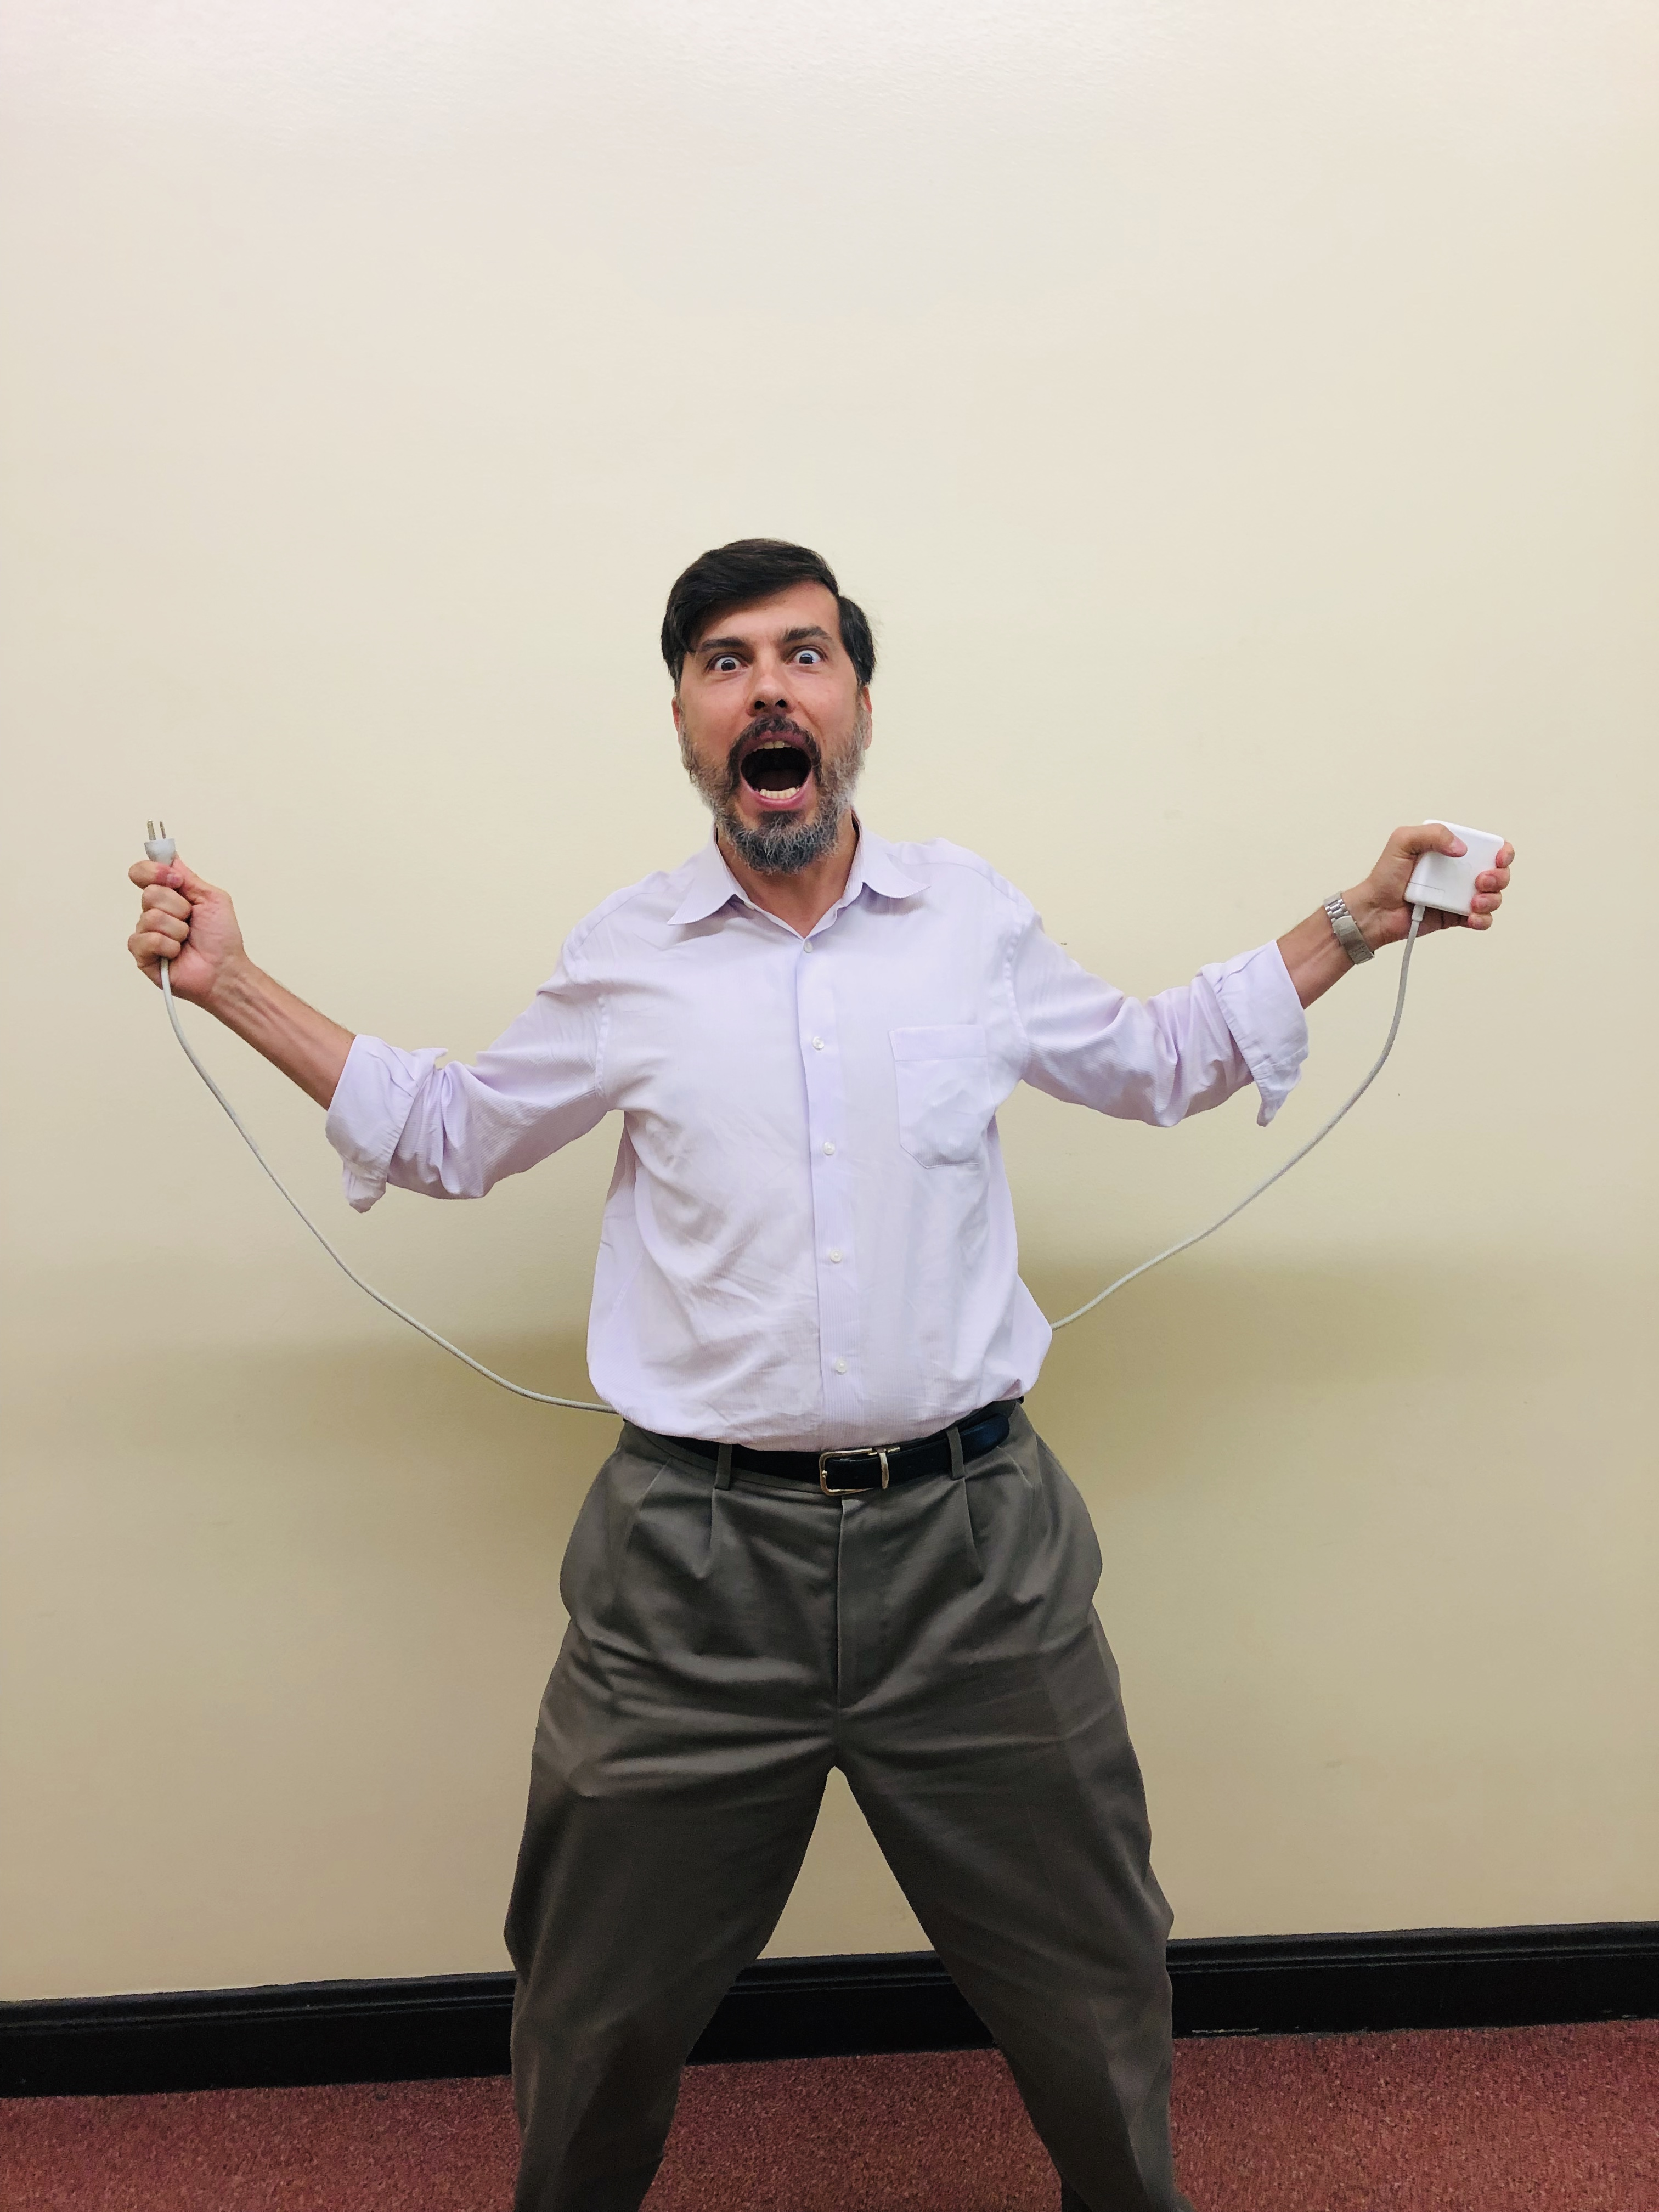
\includegraphics[width=0.45\textwidth]{figures/ab.jpg}
     \caption{Prof. Bayen's laptop wire curve}
 \end{figure}
 \begin{figure}[H]
  \centering
  \begin{minipage}[b]{0.45\textwidth}
    \includegraphics[height=9cm]{figures/catenary.png}
    \caption{GSI Theo's laptop wire curve}
  \end{minipage}
  \hfill
  \begin{minipage}[b]{0.45\textwidth}
    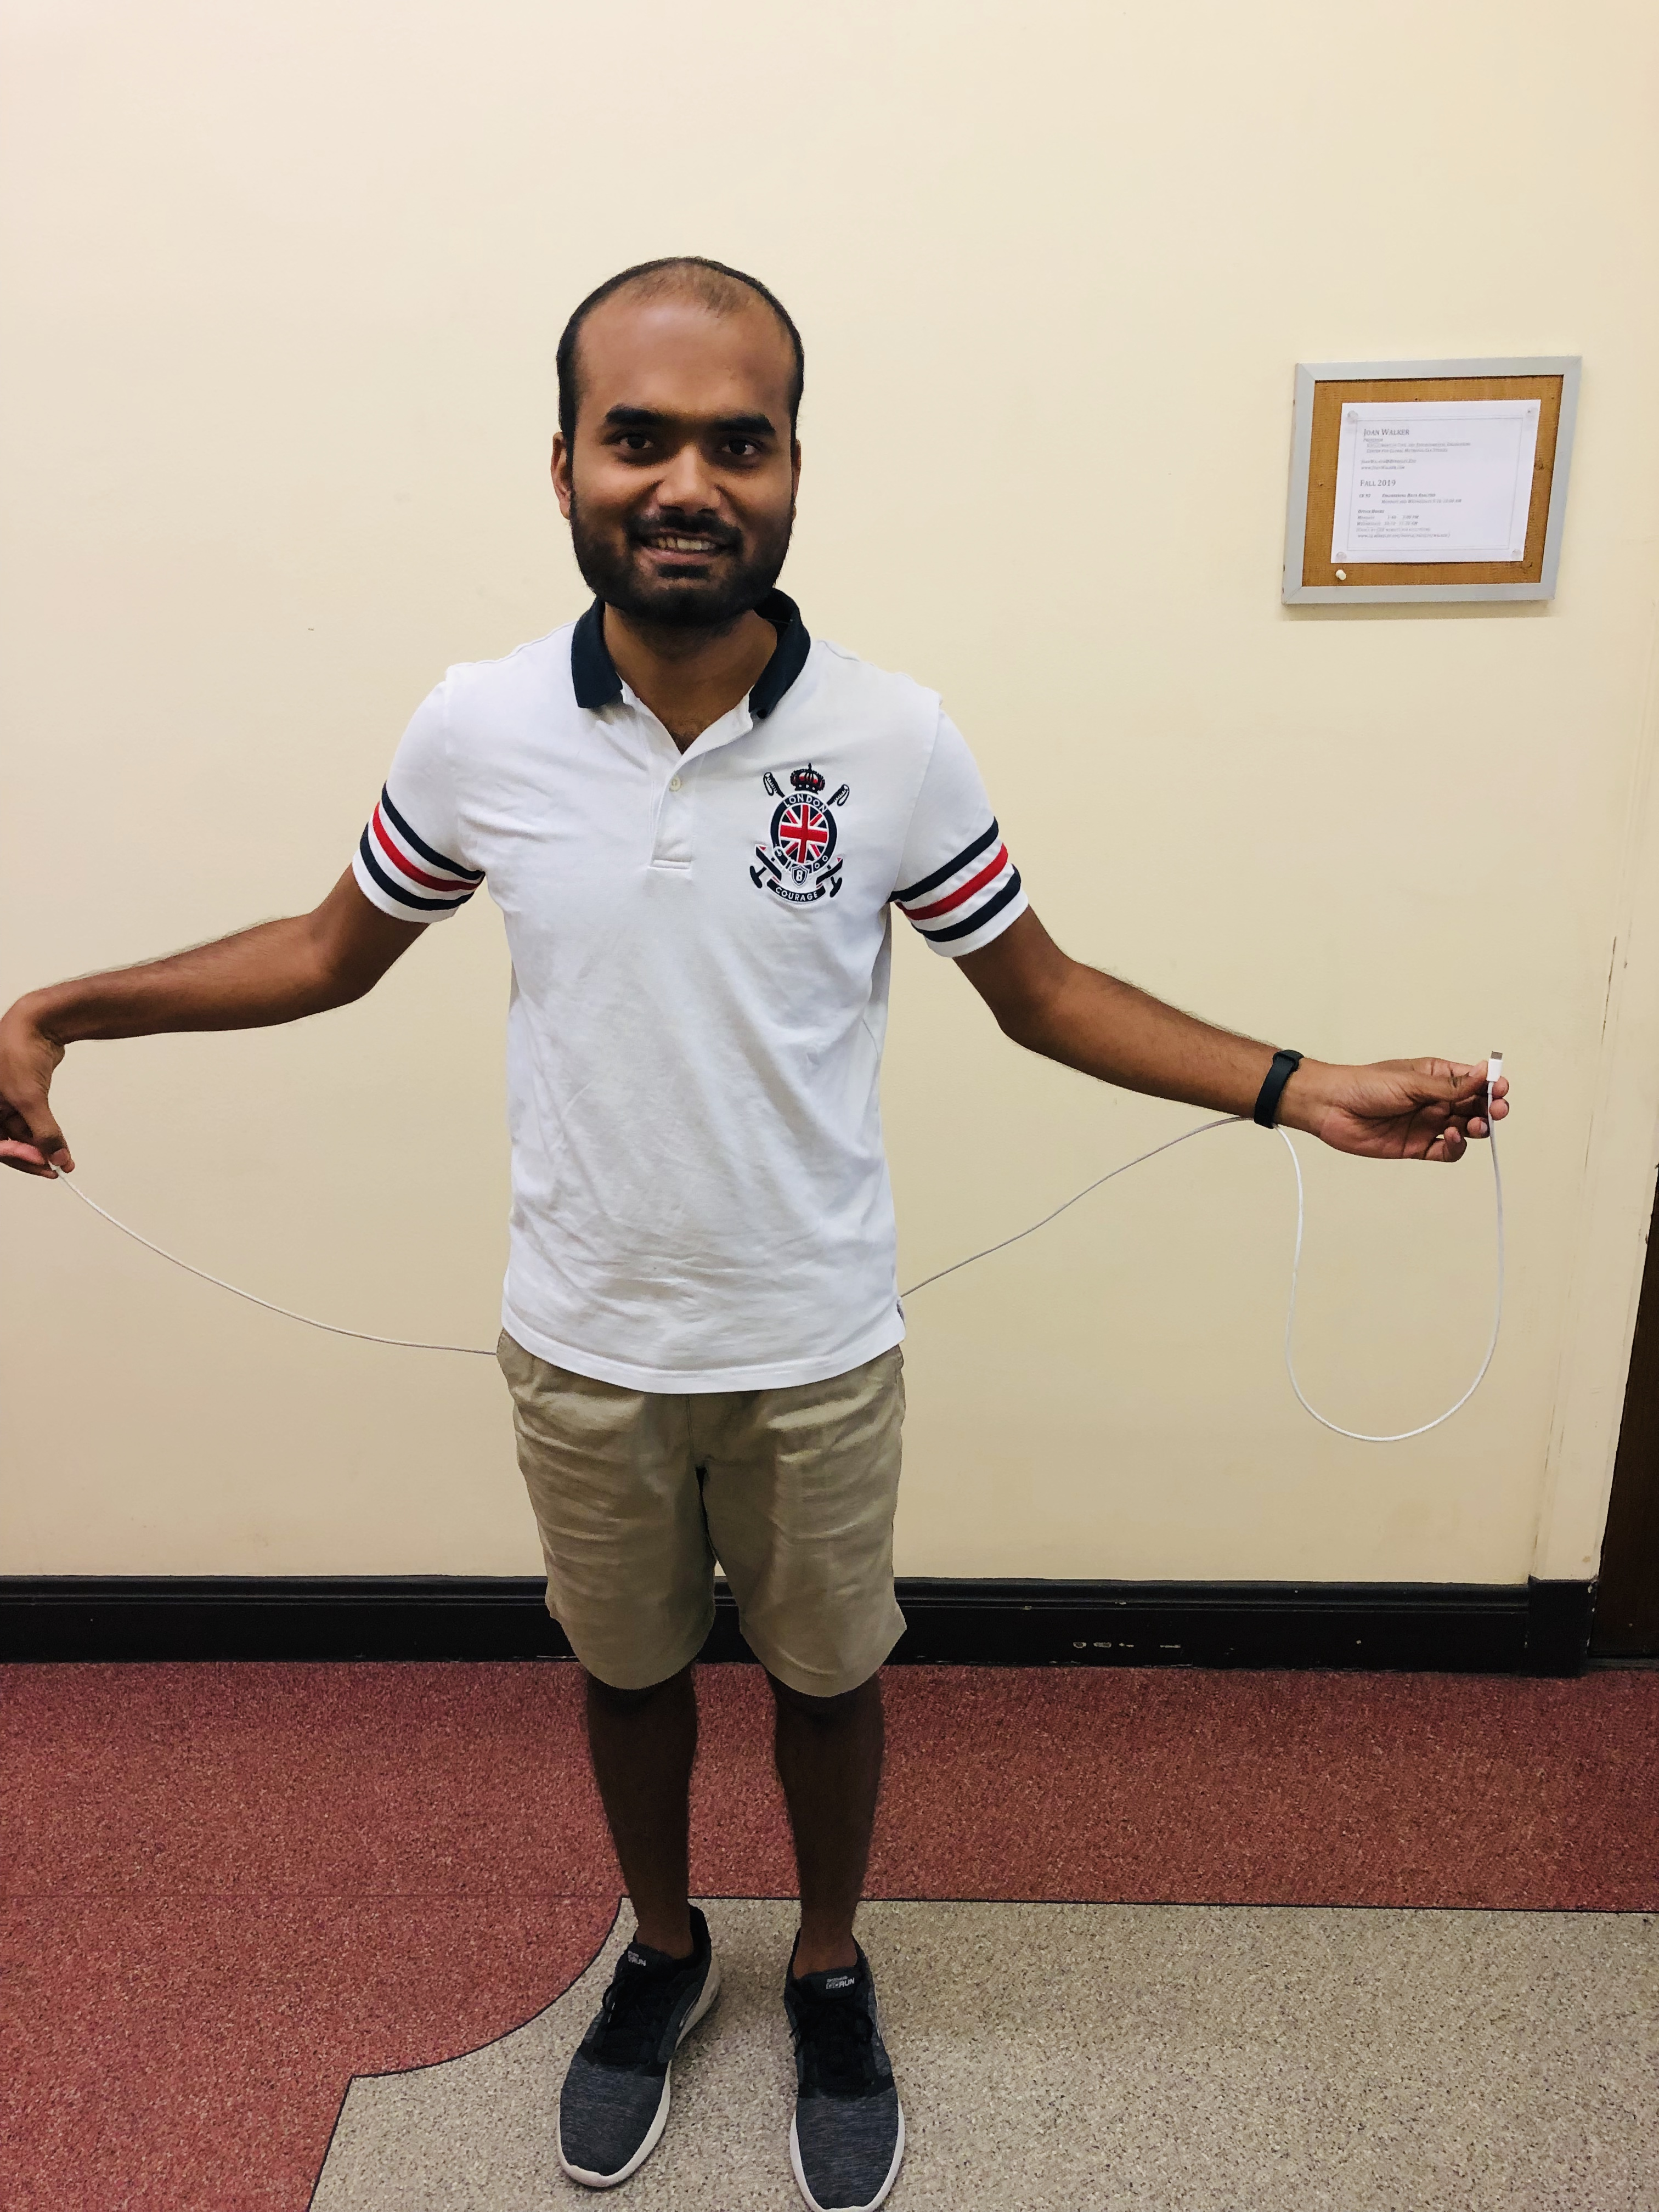
\includegraphics[height=9cm]{figures/hpd.jpg}
    \caption{GSI Hari's laptop wire curve}
  \end{minipage}
\end{figure}
\begin{figure}[H]
  \centering
  \begin{minipage}[b]{0.45\textwidth}
    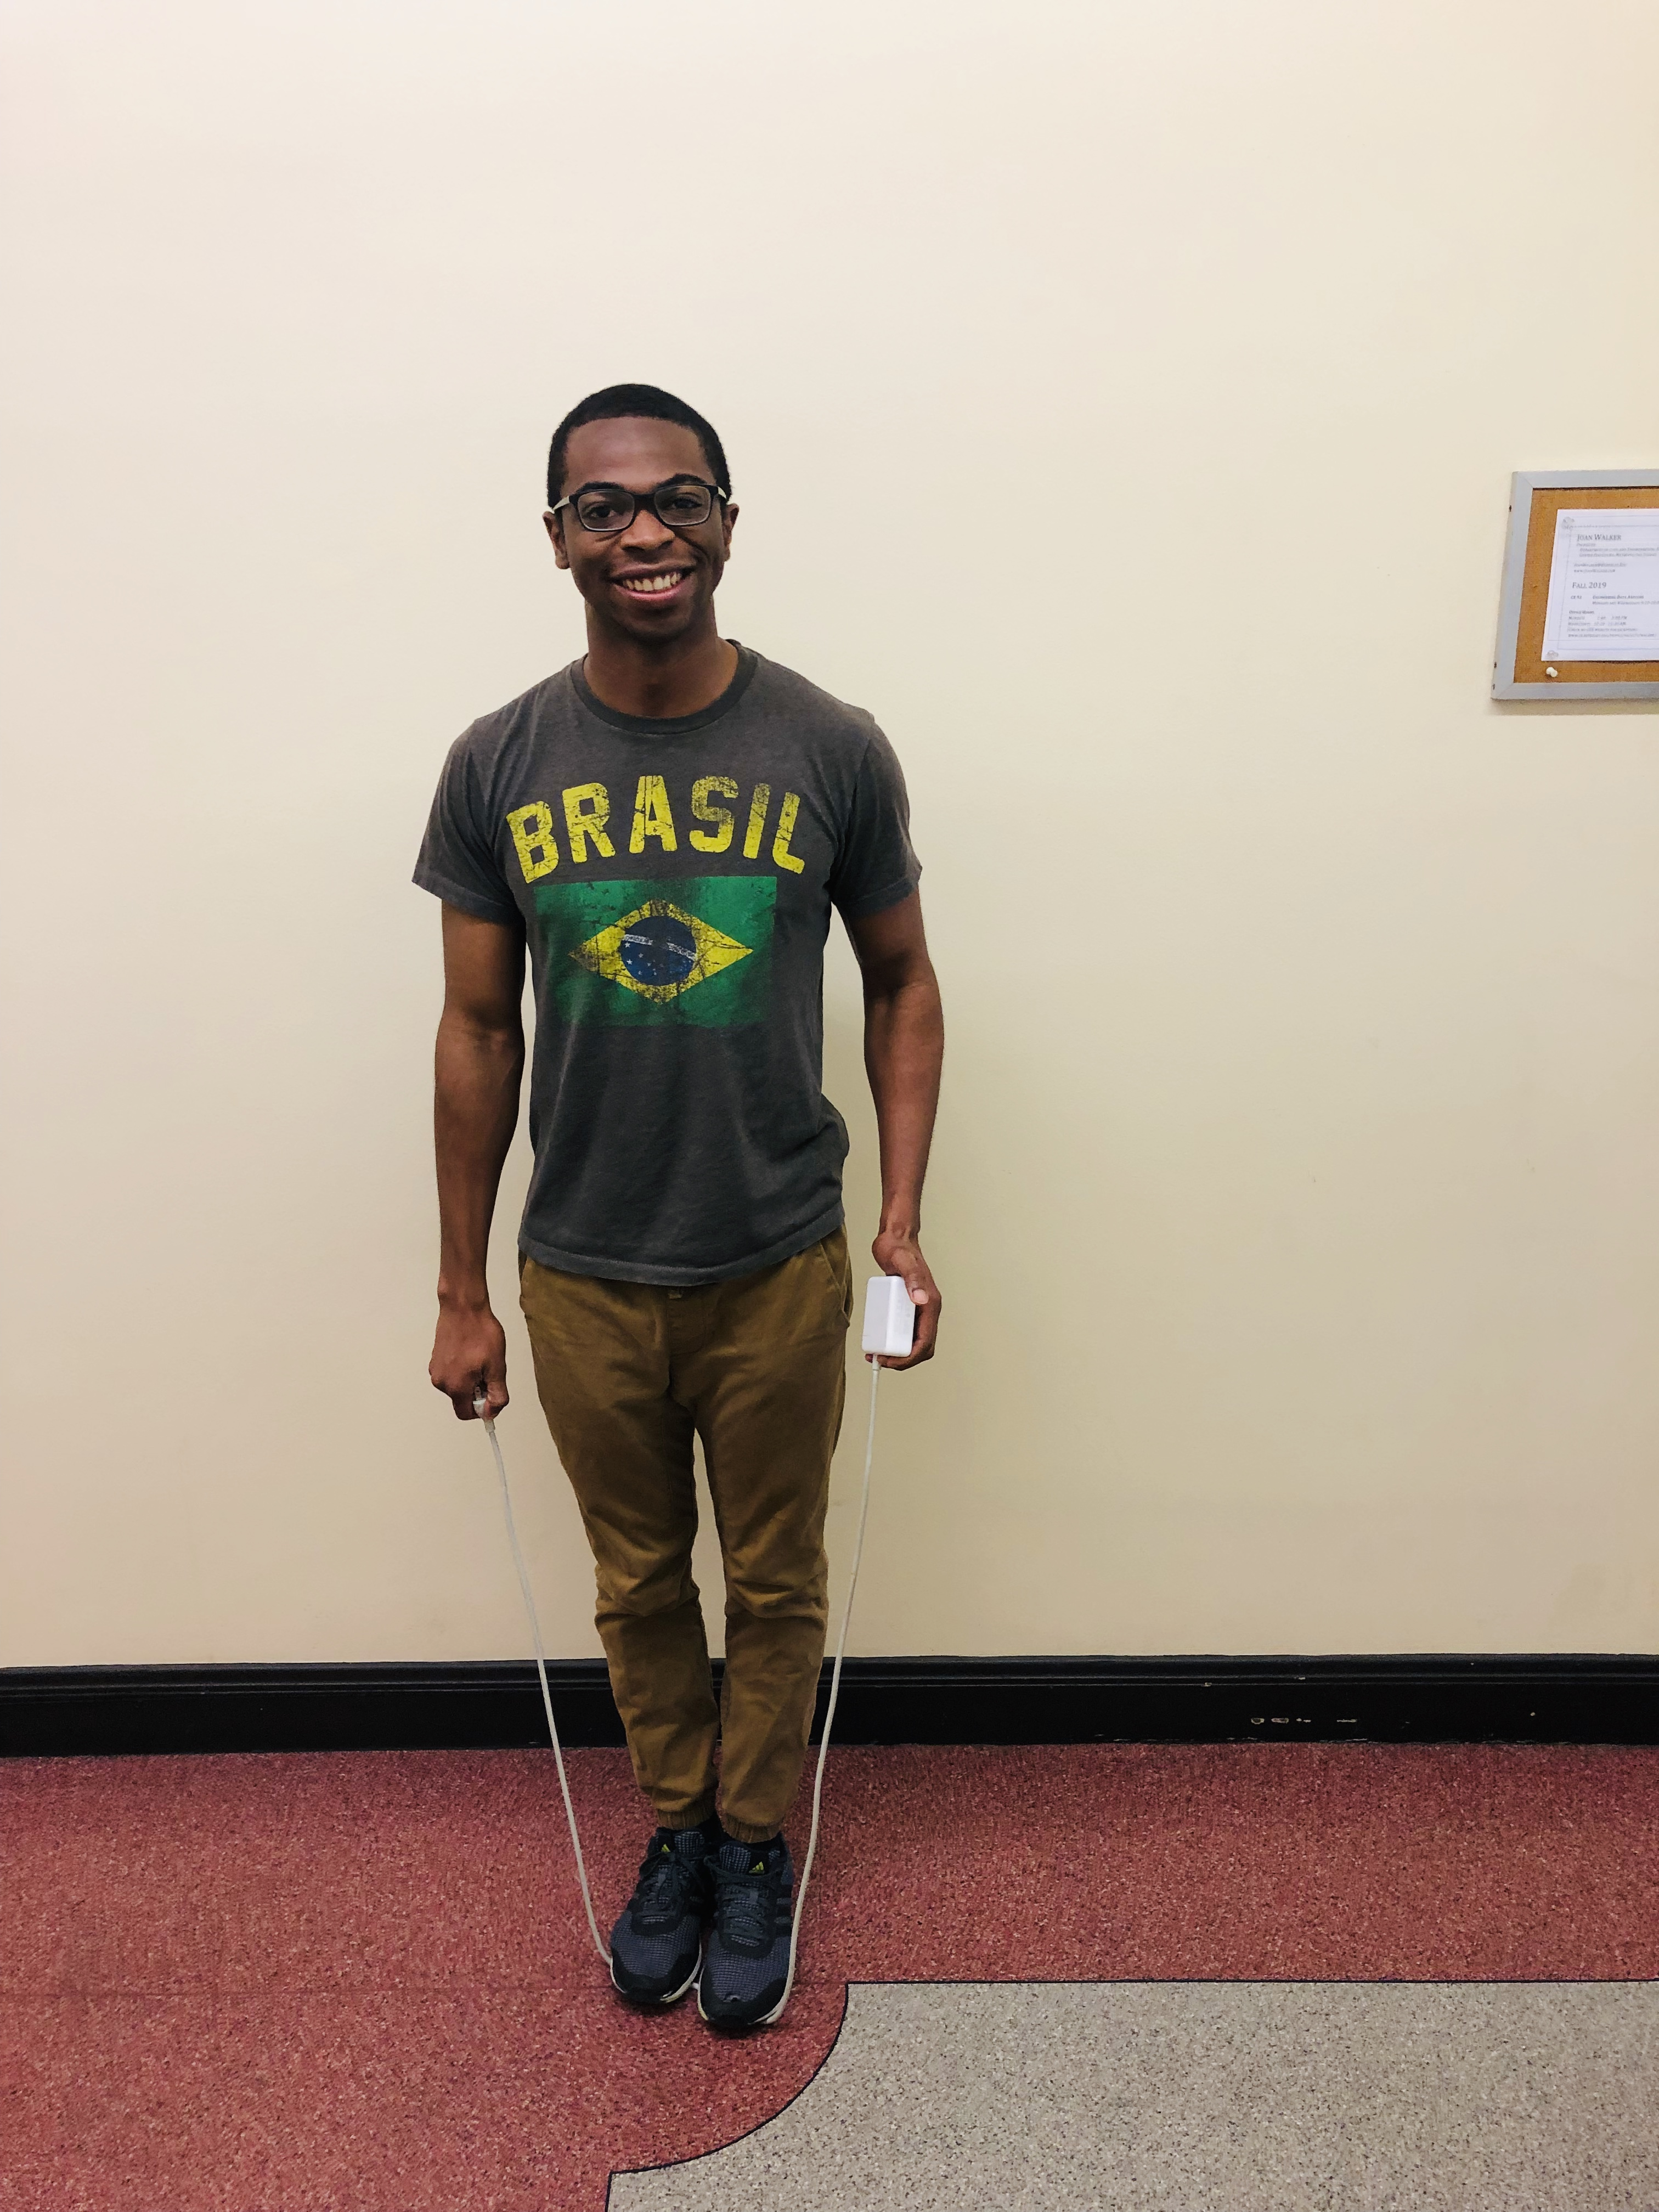
\includegraphics[height=9cm]{figures/oa.jpg}
    \caption{GSI Oladapo's laptop wire curve}
  \end{minipage}
  \hfill
  \begin{minipage}[b]{0.45\textwidth}
    
\includegraphics[height=9cm]{figures/sa.jpg}
    \caption{GSI Sukrit's laptop wire curve}
  \end{minipage}
\end{figure}
    \sol{
    \item
\[
g(x) = \begin{bmatrix}
x_1^2/x_2 \\
\log(x_3) \sin(x_1/x_3)
\end{bmatrix}
\]
    }

\end{enumerate}
